\documentclass[12pt]{article}

\usepackage[utf8]{inputenc}
%\usepackage[frenchb]{babel}
\usepackage[T1]{fontenc}
%\usepackage{t1enc}
\usepackage{longtable}
\usepackage{layout}
\usepackage[top=2.8cm, bottom=2.8cm, left=2.8cm, right=2.8cm]{geometry}
\usepackage{setspace}
\usepackage{graphicx}
\usepackage{libertine}
\usepackage{sidecap}
\usepackage{caption}
\usepackage{fancyhdr}
\usepackage{titlesec}
\usepackage{subfig}
\usepackage{placeins}
\usepackage{multirow}
\usepackage{listings}
\usepackage{dsfont}
\usepackage{amsmath}
\usepackage{changes}


\begin{document}
\title{The Sir Ivan Fire: observed pyroCb formation and features, ground-plume coupling and coldfront impact - Article Frame}

\maketitle


\section{Abstract}

\section{Introduction}
Points to be covered:
\begin{itemize}
\item Presentation of the fire (date, quick overview of the meteorological context, area burnt, pyroCb presence)
\item Context and objectives
\begin{itemize}
\item Extreme fire with pyroCb generation with a lot of observations: good case study
\item Focus of the study: We apply known methods (uss of doppler radar to get axial/absolute doppler velocity and turbulence) to a different kid of plume: a pyroCb
\item focusing on plume study, the goal is to generalize to some extent what kind of turbulence/vorticity can be expected in a pyroCb.
\end{itemize}

\item State of the art:

\begin{itemize}
\item Radar Doppler are widely used in storm studies to detect large vortices/turbulence (couple of references to add)
\item PyroCb have been studied in Australia and America through several case studies (Chislom fire, 2013 Rim fire), mostly via satellite.
\item Vortices often developp within the plume at different scales (Development of vortices on prescribed fires, review of vortices in wildland fire), but these vortices have not been watched many times (Smoke Column observation from two forests fires using doppler lidar and doppler radar)
\item The turbulence field within a pyroCb has not been studied
\end{itemize}

\end{itemize}

\section{Methods used}
\begin{itemize}
\item Namoi radar characteristics (WSR 74 S band doppler), highlight on the spec width
\item NCAR Turbulence Detection Algorythm (to get the turbulence field from the reflectivtyand the spec width)
\item Single Doppler algorythm
\end{itemize}

\section{Results}
\subsection{Meteorological and ground context}
\paragraph{Meteorological context}~\\

Main points:
\begin{itemize}
\item Perfect ground/low-level condition for an extreme fire behaviour: surface winds, RH, Temp 
\item Good pyrocb condition: Mid-level moisture/upper-level instability 
\item a coldfront was present, link to even bigger event
\end{itemize}

\textbf{Figure here} to summarize the meteorological conditions: The center of the figure could be a couple of top views of the area  at key time with the surface winds and the coldfront passage, the sides of the figure could be availale soundings to see the stability of the atmosphere

\paragraph{Ground fire results}~\\

Main points:
\begin{itemize}
\item Show the dramatic increase in spreadinding/intensity on sunday afternoon
\end{itemize}


\textbf{\ref{ground_fire} here}: The center will be the top view of the burnt area evolution, and a graph will the FRP (fire rate power) and the burnt area over time would complete it.



\subsection{Plume Structure and developments}

Main points:
\begin{itemize}
\item The plume has three steps of development
	\begin{enumerate}
	\item Before pyroCb
	\item After pyroCb/ before ColdFront
	\item After Coldfront
	\end{enumerate}
\item The plume has a structure resulting of both buoyancy driven effects and wind driven effects. 
\item Structure description:
	\begin{itemize}
	\item Vertical column (buoyancy driven)
	\item Horizontal spread at low/mid elevations in the south east (wind driven)
	\item Horizontal spread at low elevation in the north direction after the coldfront (wind driven)
	\end{itemize} 
	\textbf{Figure \ref{3steps} here}: himawari and 2-3 reflectivity signatures and 3 key timesteps to show the pyroCb structure and its evolution
	
\item PyroCb impact on the plume (top height and reflectivity distribution) \textbf{Figure here}: top height over time and reflectivity distribution at key time steps {\color{red} Note: I still have to plot the reflectivity distribution in the whole volume}

\item Litghnings (?)
\end{itemize}

\subsection{Turbulence/ Vortices within the plume}

Main points:
\begin{itemize}
\item Before the pyroCb: expected features:
	\begin{itemize}
	\item The divergence line on the doppler plots follow the center line: no large vortices
	\item The turbulences are maximum at the edges of the plume 
	\end{itemize}
\item After the pyroCb we see unexpected features:
	\begin{itemize}
	\item Large vortices signatures along the centerline of the plume
	\item Turbulence field disturbed, maxima o turbulence along the centerline of the plume
	\item The center of the plume presents both large scale (cf doppler signature) and smaller scale (cf turbulence field) vortices.
	\end{itemize}
	
\textbf{Figure here}: Showing over 1 time step of  the "normal" velocity field/turbulence and a series of the unexpected turbulence and vortices (3-4 between 17:20 and 18:10 to show the motion of the vortices)
\end{itemize}
\section{Discussions}

\subsection{Discussion about the pyroCb generation}
The atmospheric/ground conditions are they consistent with the litterature ? {\color{red}Note: The point would be to show that our case is not that different from others, to then support a generalization}

\subsection{Analysis of the vortices/ turbulence within the plume}
What is the part of the pyroCb ? what is the part of the coldfront ? can some other parameters explain the unexpected features ?
{\color{red} Note: this part is not clear to me yet, it is definitely where there still is the more to do}


\section{Conclusion}
{\color{red} Note: Will depend on the discussion}
\section{References}

\section{figures}

{\color{red} Note: These figures are not finished yet, figure \ref{ground_fire} needs some more data from the NFS, figure \ref{3steps} needs some presentation work from me, figure \ref{tur_vel} might need additional elevation, and maybe the single doppler field. Since this last figure is crucial for the article, I was considering splitting it in two one for the doppler velocity, the other part for the turbulence.}

\vspace{0.5cm}

{\color{red} Note: Two more figures are to be done as well: The one presenting the atmospherical condition (I m waitng for data front the NFS, and the one presenting the top height and the reflectivity distribution)}

\begin{figure}[position]
   \caption{\label{ground_fire} Fire spread during the event (main), area burnt and FRP over time (bottom right).   {\color{red} Note: the point of this figure is to show the massive increase in area and FRP on sunday. The graph does not display the right information yet (I m waiting for the ground data from the NFS)} }
   \includegraphics[width=\textwidth]{figures/ground_fire.png}
\end{figure}

\begin{figure}[position]
   \caption{\label{3steps} Evolution of the plume on sunday. The each column corresponds to a time step: the first is 15:00pm, before the pyroCb, the second is 17:00, after the apparition of the pyroCb and during the coldfront passage, the last columns corresponds to 18:10pm, after the coldfront passage. The first line shows the visible Himawari view, and the two other rows the reflectivity signature for 0.5 and 1.8 degree of elevation.   {\color{red} Note: the point of this figure is to show the plume evolution: first a soft expansion to the south-east, then the apparition of the pyroCb, and finally the coldfront creating a new expansion to the north east, but only at low level} }
   \includegraphics[width=\textwidth]{figures/3main_steps.png}
\end{figure}

\begin{figure}[position]
   \caption{\label{tur_vel} Axial Doppler velocity and turbulence field at four time steps: 15:40, before the apparition of the pyroCb ; 17:00, during the pyroCb event, and at the begining of the large vortices signatures and the move of the maximum of turbulence toward the centre ; 17:50 and 18:10 with the motion toward south east of the large vortex. {\color{red} note: the point of this figure is to show The apparition and the development of the vortexes and the turbulence displacement. An interesting featur is that the vortex doesn't follow the coldfront wind direction, but the mid level wind direction. So I m considering adding another radar elevation to show that the same signature on vortex and turbulence are present as well} }
   \includegraphics[width=\textwidth]{figures/vel_turb.png}
\end{figure}
\end{document}